% ============================================================
%  TERM PROJECT – PROPOSAL (template)
%  Databases · THGA Bochum
%
%  How to use:
%    1. Copy this folder into your own repository.
%    2. Replace every  <<< ... >>>  placeholder with your content.
%    3. Build with  `make`  (see the Makefile / README).
%    4. Send the resulting PDF to the lecturer and wait for approval.
% ============================================================
\documentclass[11pt,a4paper]{article}

\usepackage{thga-db}
\usepackage{caption}   % enables \captionof inside minipages
\usepackage{seqsplit}  % allows line-breaking inside long unbroken \texttt strings (e.g. API paths)

% ----- Placeholder figure (delete once you insert a real image) ----
% Draws a labelled box you can swap for \includegraphics later.
% Usage: \placeholder{width}{height}{label text}
\usetikzlibrary{positioning}
\newcommand{\placeholder}[3]{%
  \begin{tikzpicture}
    \node[draw=THGABlau!45, fill=THGABlau!5, very thick, rounded corners=2pt,
          minimum width=#1, minimum height=#2, align=center, inner sep=6pt,
          text=THGABlau!75, font=\small\itshape] {#3};
  \end{tikzpicture}%
}

% ----- Fill in your metadata -------------------------------
\renewcommand{\thgaKurs}{Databases}
\renewcommand{\thgaDatum}{Summer Term 2026}
\newcommand{\authorName}{Anton Möller}
\newcommand{\projectTitle}{Prevently Health Checkup Management System}

\begin{document}
\thispagestyle{empty}
\thgaTitel{Term Project – Proposal}{\projectTitle}

\begin{infobox}
\textbf{Author:} \authorName \\
\textbf{Module:} Introduction to Database Management Systems · THGA Bochum \\
\textbf{Submitted to:} Stephan Bökelmann · \href{mailto:sboekelmann@ep1.rub.de}{sboekelmann@ep1.rub.de} \\
\textbf{Target size:} about 6 pages
\end{infobox}

% ============================================================
\section{Application domain and motivation}
% ============================================================

I would like to build an application that allows users to manage and track their medical checkups and appointments based on
their age, gender and insurance coverage. Most people don't have a good overview of their needed checkups and if the costs are 
covered by their insurance. I had this idea already some time ago, but never had the time beside work to implement it. Now I would like to use this project 
as a starting point to implement a first mvp version. With this version a user should see which checkups are due and if they're covered by their insurance.
He should also be able to check which doctors are available for this checkup and add his appointment to the system.
It should also be possible to check which doctor can perform which checkups and the user should be able to add his own checkups
from the past and doctors to the system. The database models insurance providers and their covered services, doctors and their specializations, 
a catalog of preventive-care types with age- and gender-specific rules to allowing the system to automatically derive which check-ups 
are currently due for a given user. One example usage scenario is a user who wants to know which checkups are recommended for 
his age and gender, and which of those checkups are covered by his insurance. My database will allow the user 
to show the checkups that should be done for the user age. This could be done for some different users but this version doesn't support specific users.
If a user already did the checkup, then this one doesn't appear anymore as a recommended checkup. The Appointment feature will in this 
version only a feature that allows the user to add appointments to the system, which doesn't include collision detection or other advanced 
features because I think this could be too much work for this project. This appointment will be stored in the database and the user can see it in the system. 
This application is intended to be a prototype and a authentication, encryption and different user roles won't be implemented in this version because I think this will be
too much work for the time assigned to this project but I would be very happy to also hear some tips afterwards like we
already had in the lessons before.

\newpage
% ============================================================
\section{Data model -- ER sketch}
% ============================================================

\begin{figure}[ht]
  \centering
  % Replace the placeholder with: \includegraphics[width=0.85\linewidth]{er-sketch.jpg}
  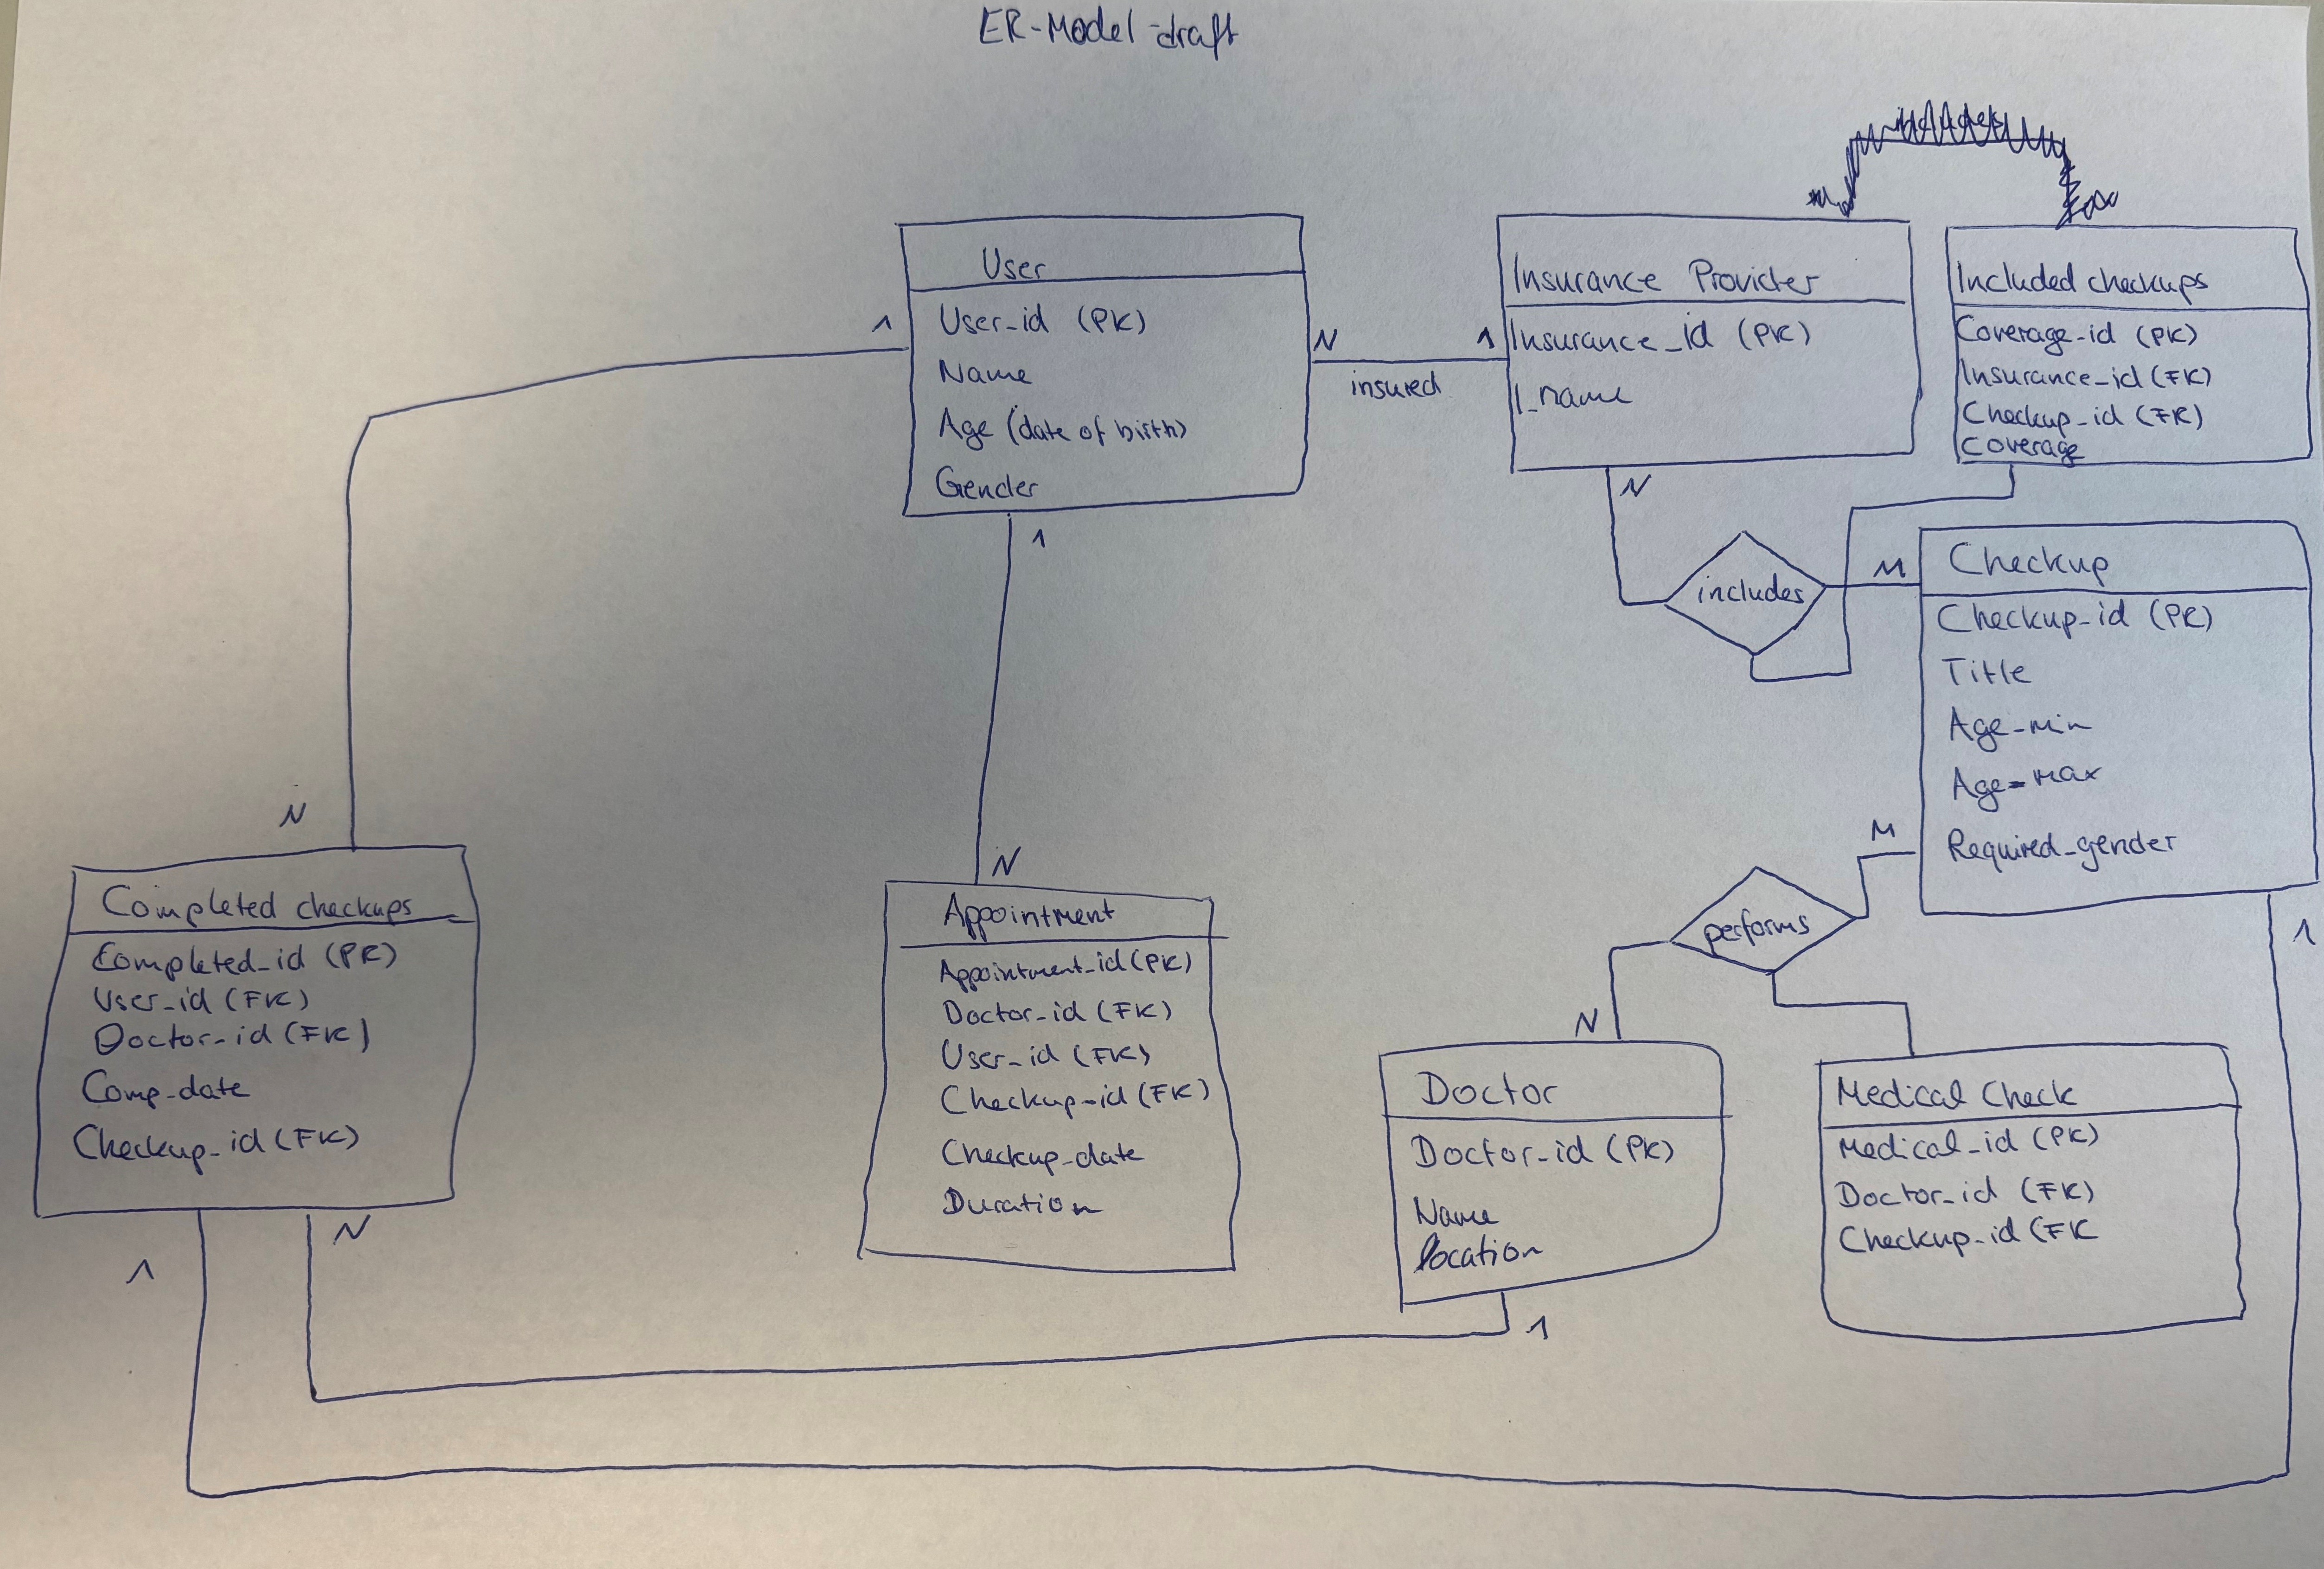
\includegraphics[width=0.85\linewidth]{assets/ERdraft.jpg}
  \caption{ER sketch of the health-check data model: entity types, key
  attributes, relationships and cardinalities (at least one N:M).}
  \label{fig:er}
\end{figure}

Figure~\ref{fig:er} shows my hand-drawn ER sketch of the data model. The central entity types are \texttt{User}, \texttt{Insurance Provider},
\texttt{Checkup} and \texttt{Doctor}. The User entity only has a few attributes like name, age, gender. The first N:M relationship
is between the \texttt{Insurance Provider} and the \texttt{Checkup} entity. Another key entity is the \texttt{Checkup}, which has attributes
like the age\_min, age\_max and required gender. This information could be used to determine if a checkup is due for a user. Then there is 
also the \texttt{Completed checkups} entity, which stores the Completion date and the user\_id and checkup\_id as a foreign key from the
\texttt{User} with the N:1, the \texttt{Doctor} with N:1 and the \texttt{Checkup} entity with 1:1 cardinality.
From the \texttt{Insurance Provider} entity there is also a N:1 relationship to the \texttt{User} entity because normally one person only 
has one insurance provider (without any additional providers) and a \texttt{Insurance Provider} has multiple \texttt{User}.
This is N:M because an insurance provider could cover many checkups and a checkup could be covered by many different insurance providers. 
The second N:M relationship is between the \texttt{Doctor} and the \texttt{Checkup} entity. I've chosen this relationship because a checkup 
could be performed by many different doctors and in most of the cases a doctor could also perform different checkups.


% ============================================================
\section{From model to schema}
% ============================================================


\begin{itemize}
  \item \texttt{User}(\underline{User\_id}, Name, Date\_of\_birth, Gender, \dots)
  \item \texttt{Insurance\_provider}(\underline{Insurance\_id}, I\_name, \dots)
  \item \texttt{Checkup}(\underline{Checkup\_id}, Title, Age\_min, Age\_max, Required\_gender, \dots)
  \item \texttt{Doctor}(\underline{Doctor\_id}, Name, Location, \dots)
  \item \texttt{Completed\_checkups}(\underline{Completion\_id}, \emph{User\_id}, \emph{Doctor\_id}, \emph{Checkup\_id},  Comp\_date, \dots)
  \item \texttt{Included\_checkups}(\underline{Coverage\_id}, \emph{Insurance\_id}, \emph{Checkup\_id}, Coverage, \dots)
  \item \texttt{Medical\_check}(\underline{Medical\_id}, \emph{Doctor\_id}, \emph{Checkup\_id}, \dots)
  \item \texttt{Appointment}(\underline{Appointment\_id}, \emph{Doctor\_id}, \emph{User\_id},  \emph{Checkup\_id}, Checkup\_date, Duration, \dots)
\end{itemize}

\textbf{Normalisation.} 

The schema is normalized to at least Third Normal Form (3NF). 
Each table represents a single entity type and contains only attributes that are directly dependent on its primary key.


% ============================================================
\section{API design}
% ============================================================

The table below lists the planned FastAPI endpoints. Read endpoints are open;
write endpoints require the \texttt{X-API-Key} header.

\renewcommand{\arraystretch}{1.2}
\begin{tabularx}{\linewidth}{@{}p{1.3cm}p{4.3cm}X@{}}
\toprule
\textbf{Method} & \textbf{Path} & \textbf{Purpose} \\
\midrule
\texttt{GET}  & \texttt{\seqsplit{/checkups}} & Lists all checkup types with their age/gender rules. \\
\texttt{GET}  & \texttt{\seqsplit{/users/\{id\}/due-checkups}} & Checkups due for a user (JOIN \texttt{Checkup} + \texttt{Completed\_checkups}, filtered by age/gender and completion status). \\
\texttt{GET}  & \texttt{\seqsplit{/users/\{id\}/completed-checkups}} & Checkups already completed by a user (JOIN \texttt{Completed\_checkups} + \texttt{Checkup} + \texttt{Doctor}). \\
\texttt{GET}  & \texttt{\seqsplit{/checkups/\{id\}/coverage}} & Insurance providers covering a checkup (JOIN \texttt{Checkup} + \texttt{Included\_checkups} + \texttt{Insurance\_provider}). \\
\texttt{GET}  & \texttt{\seqsplit{/doctors/\{id\}/checkups}} & Checkups a doctor can perform (JOIN \texttt{Doctor} + \texttt{Medical\_check} + \texttt{Checkup}). \\
\texttt{GET}  & \texttt{\seqsplit{/checkups/\{id\}/doctor-count}} & Aggregation: number of doctors offering this checkup (\texttt{COUNT} over \texttt{Medical\_check}). \\
\texttt{GET}  & \texttt{\seqsplit{/checkups/\{id\}/doctors}} & Doctors who can perform a checkup, optionally filtered by location (JOIN \texttt{Checkup} + \texttt{Medical\_check} + \texttt{Doctor}). \\
\texttt{GET}  & \texttt{\seqsplit{/insurance-providers/\{id\}/checkups}} & Checkups covered by an insurance provider, with coverage rate (JOIN \texttt{Insurance\_provider} + \texttt{Included\_checkups} + \texttt{Checkup}). \\
\texttt{POST} & \texttt{\seqsplit{/checkups}} & Creates a new checkup type with its age/gender rules (requires X-API-Key). \\
\texttt{POST} & \texttt{\seqsplit{/users}} & Creates a new user (requires X-API-Key). \\
\texttt{POST} & \texttt{\seqsplit{/insurance-providers}} & Creates a new insurance provider (requires X-API-Key). \\
\texttt{POST} & \texttt{\seqsplit{/doctors}} & Creates (lists) a new doctor with their location (requires X-API-Key). \\
\texttt{POST} & \texttt{\seqsplit{/medical-checks}} & Links a checkup to a doctor who can perform it (requires X-API-Key). \\
\texttt{POST} & \texttt{\seqsplit{/completed-checkups}} & Logs a completed checkup for a user (requires X-API-Key). \\
\texttt{POST} & \texttt{\seqsplit{/included-checkups}} & Links a checkup to an insurance provider's coverage (requires X-API-Key). \\
\texttt{POST} & \texttt{\seqsplit{/appointments}} & Creates an appointment with a doctor for a checkup (requires X-API-Key). \\
\bottomrule
\end{tabularx}

% ============================================================
\section{Frontend prototype (hand sketches)}
% ============================================================

% The four boxes below are placeholders. Replace each \placeholder{...} with
% \includegraphics[width=\linewidth]{your-sketch.jpg} and keep the \captionof.
\begin{figure}[ht]
\centering
\begin{minipage}[t]{0.47\linewidth}\centering
  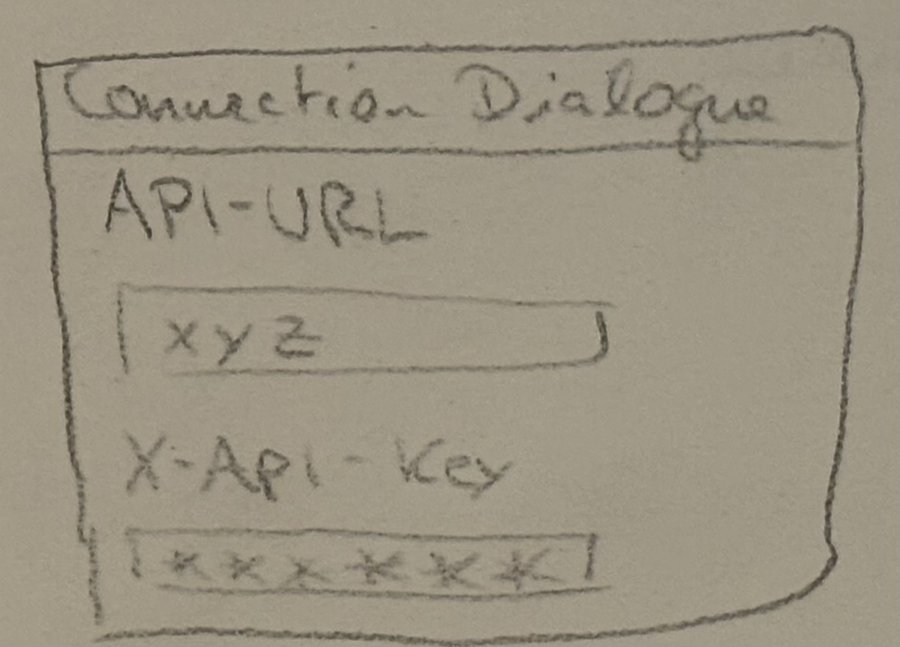
\includegraphics[width=0.85\linewidth]{assets/Connection.jpg}
  \captionof{figure}{Startup connection dialog: API URL + X-API-Key.}
  \label{fig:fe-connect}
\end{minipage}\hfill
\begin{minipage}[t]{0.47\linewidth}\centering
  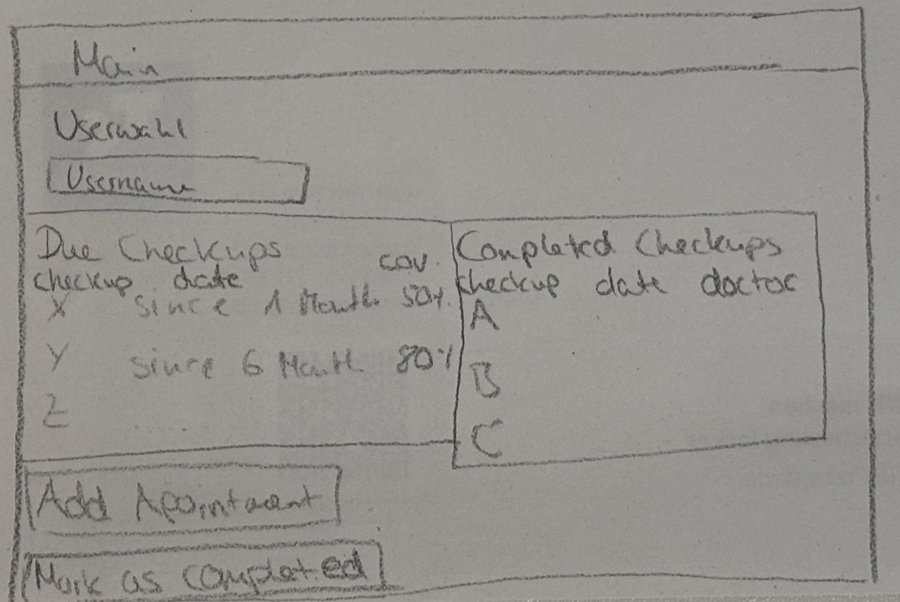
\includegraphics[width=0.85\linewidth]{assets/Main.jpg}
  \captionof{figure}{Main screen: due and completed checkups for the selected user, calls \texttt{GET /users/\{id\}/due-checkups} and \texttt{GET /users/\{id\}/completed-checkups}; ``Mark as completed'' writes via \texttt{POST /completed-checkups} for a selected checkup.}
  \label{fig:fe-main}
\end{minipage}

\vspace{1em}

\begin{minipage}[t]{0.47\linewidth}\centering
  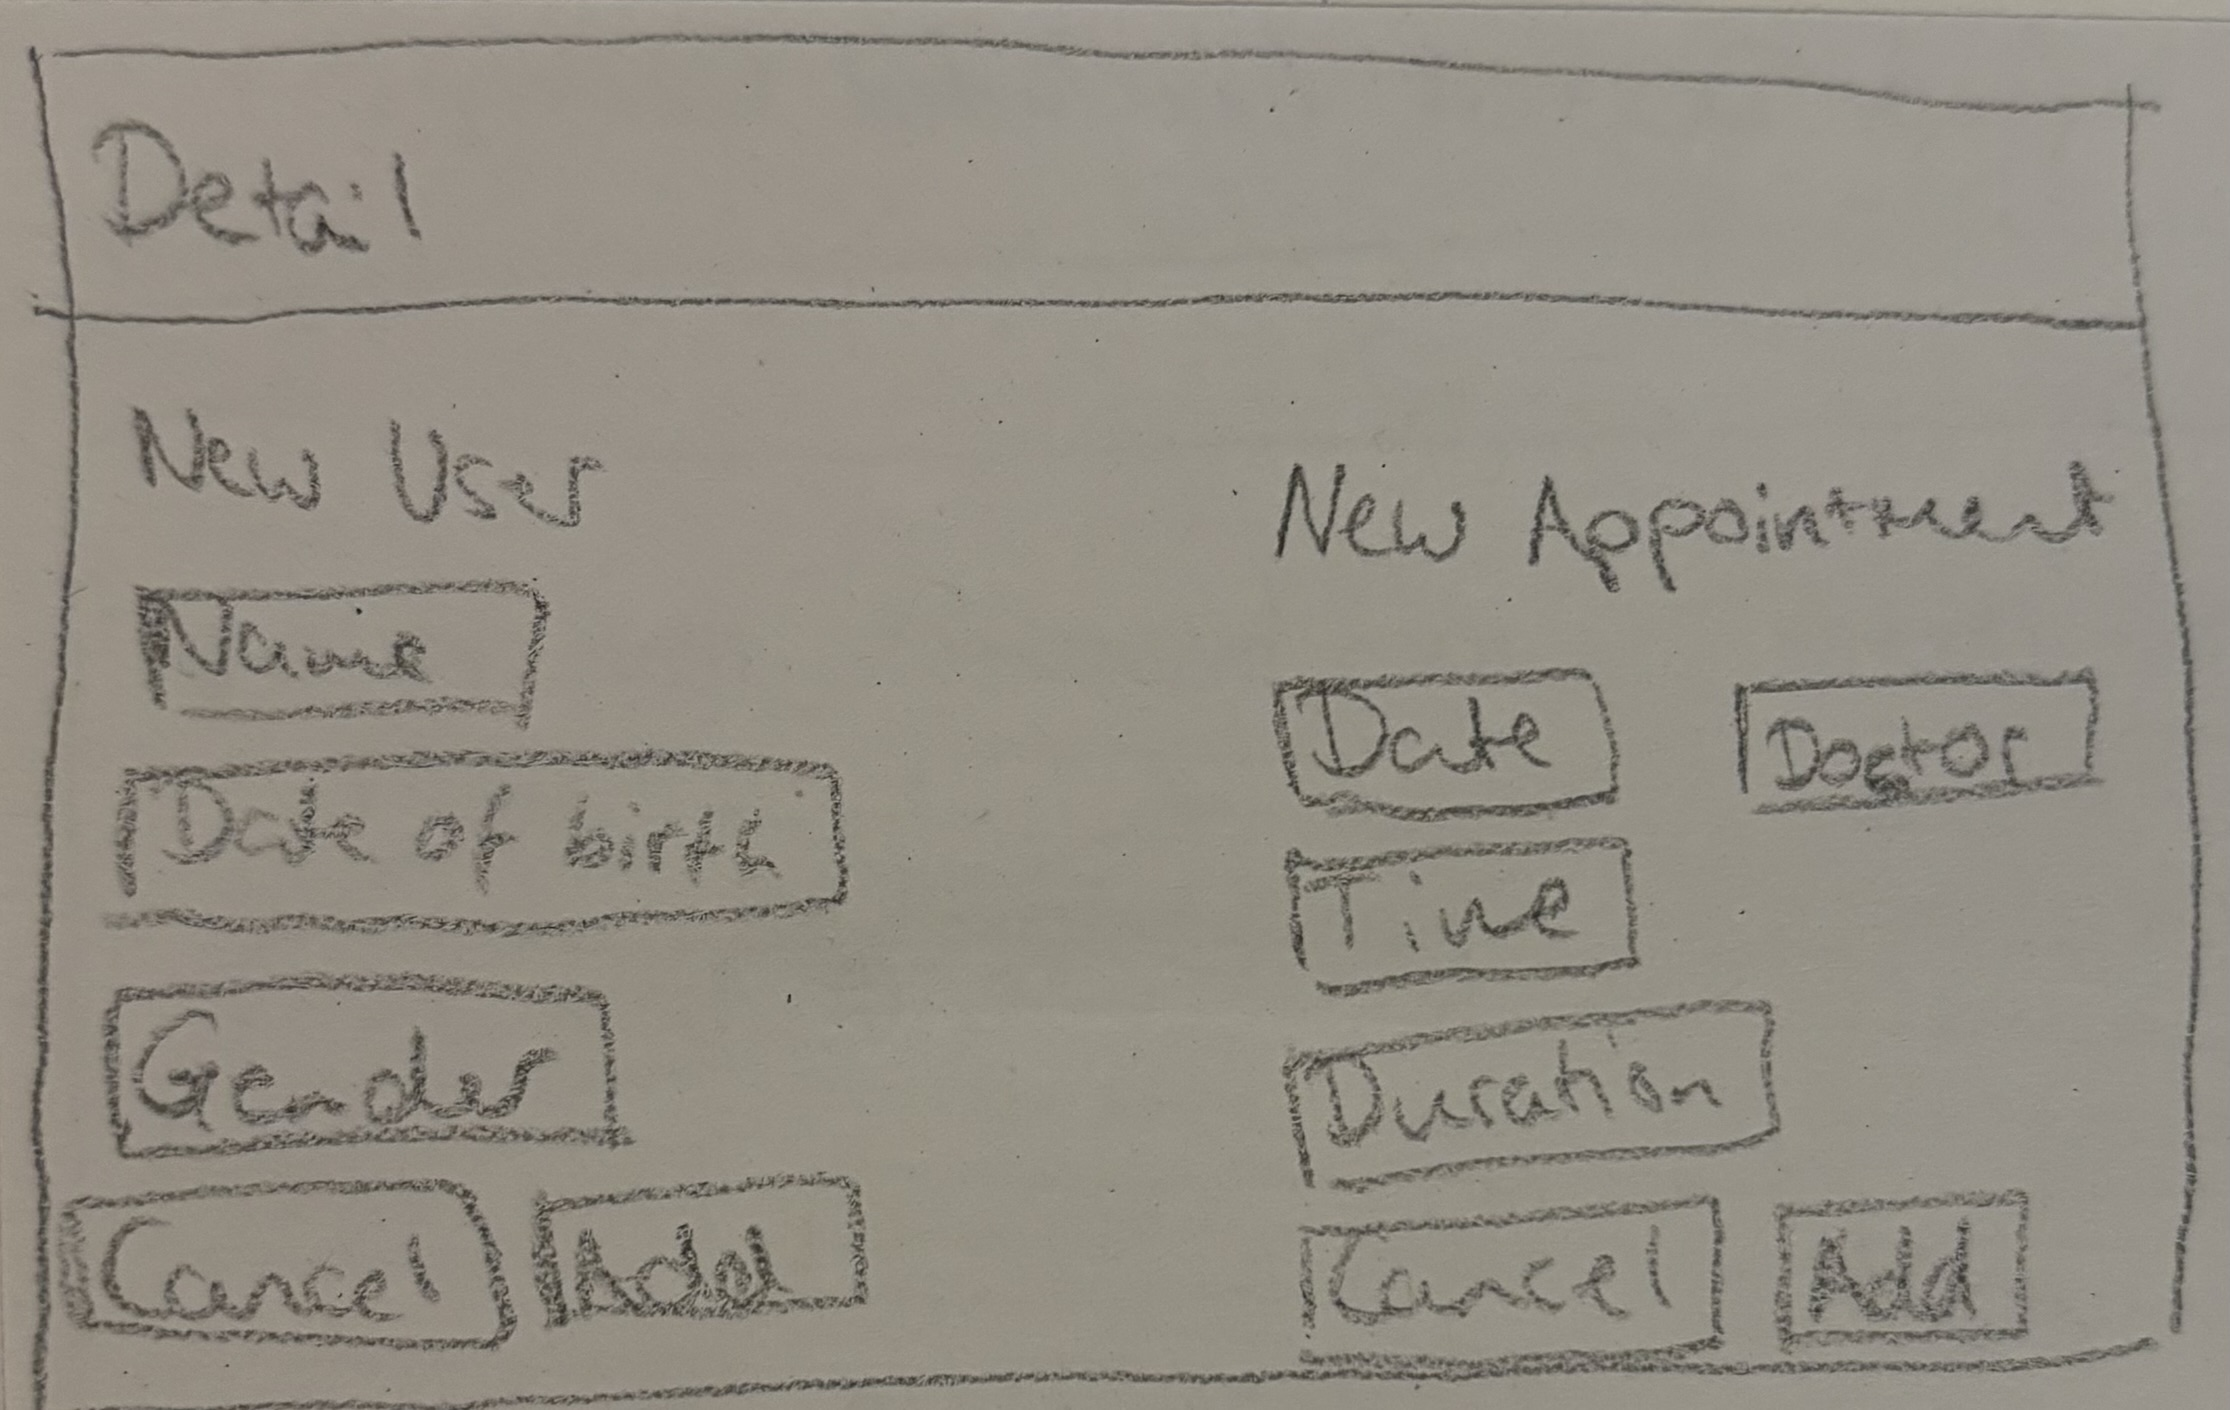
\includegraphics[width=0.85\linewidth]{assets/Deitail.jpg}
  \captionof{figure}{Detail form: create a new user via \texttt{POST /users}, and book a new appointment for the checkup selected on the main screen via \texttt{POST /appointments}.}
  \label{fig:fe-detail}
\end{minipage}\hfill
\begin{minipage}[t]{0.47\linewidth}\centering
  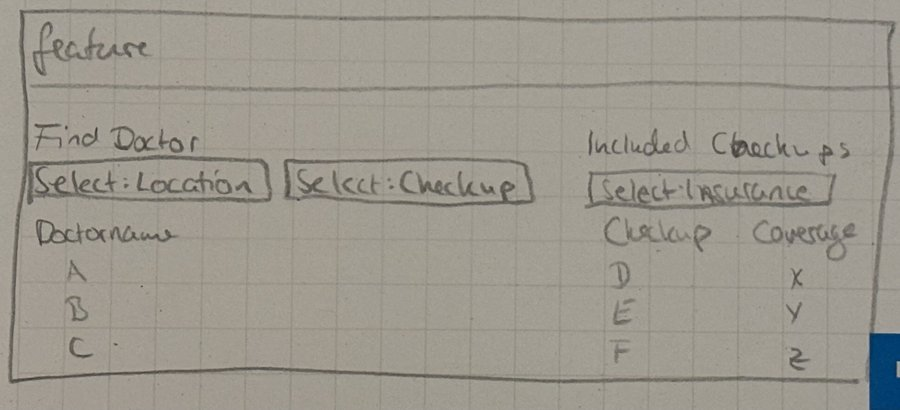
\includegraphics[width=0.85\linewidth]{assets/Feature.jpg}
  \captionof{figure}{Feature screen: find doctors for a checkup and location (\texttt{GET /checkups/\{id\}/doctors}), and list checkups covered by a selected insurance provider (\texttt{GET /insurance-providers/\{id\}/checkups}).}
  \label{fig:fe-second}
\end{minipage}
\end{figure}

Figures~\ref{fig:fe-connect}--\ref{fig:fe-second} show the four screens of the
prototype. Figure~\ref{fig:fe-connect} shows the connection dialog that
collects the API URL and X-API-Key at startup. Figure~\ref{fig:fe-main} shows
the main screen, listing due and completed checkups for the selected user, 
allowing a due checkup to be marked as completed and an appointment to be
added; Figure~\ref{fig:fe-detail} shows the detail screen used to create a new
user and to book a new appointment for the checkup selected on the
main screen. Doctors, insurance providers and checkup types are seeded with
a setup script because I think if I add them in this project, it would expand the time of roughly 40 hours.
Figure~\ref{fig:fe-second} shows the feature screen for finding doctors by
checkup and location, and for looking up which checkups a insurance
provider covers.

\newpage
% ============================================================
\section{Operation with Docker Compose}
% ============================================================

The \texttt{docker-compose.yml} defines two services: \texttt{postgres}
(official \texttt{postgres} image, with a named volume for the data directory
so the database survives container restarts) and \texttt{api} (the FastAPI
app, built from a small \texttt{Dockerfile}, running via \texttt{uv}). 
Database credentials, the database URL and the \texttt{X-API-Key}
value live in a \texttt{.env} file that is excluded via \texttt{.gitignore}
and only referenced by name in \texttt{docker-compose.yml}. 

% ============================================================
\section{Scope, milestones and risks}
% ============================================================

\textbf{Scope.} The system has 8 tables (\texttt{User}, \texttt{Insurance\_provider},
\texttt{Checkup}, \texttt{Doctor}, \texttt{Completed\_checkups},
\texttt{Included\_checkups}, \texttt{Medical\_check}, \texttt{Appointment})
and 16 endpoints (8 \texttt{GET}, including three JOIN queries and one
aggregation, 8 \texttt{POST}, all protected by \texttt{X-API-Key}). The
frontend operates a subset of these through four screens (connection, main,
detail, feature). Doctors, insurance providers and checkup types are
seeded with a setup script rather than managed through the UI, to keep the
scope more realistic for the available time.

\textbf{Milestones and schedule.} In my semester holiday I work a 40\,h/week job, so I only have a
few hours per week for this project. The schedule below spreads the work over
8 weeks (about 2 months) in small, self-contained steps instead of a few large
ones, so a busy week doesn't put the whole plan at risk and keeps it manageble.

\renewcommand{\arraystretch}{1.2}
\begin{tabularx}{\linewidth}{@{}p{1.4cm}Xp{1.8cm}@{}}
\toprule
\textbf{Week} & \textbf{Milestone} & \textbf{Est. hours} \\
\midrule
1     & Schema, migration- and seed script for master data (doctors, insurance providers, checkup types) ready & 6 \\
2     & Read endpoints implementation (\texttt{GET}, incl.\ JOINs and the aggregation) & 8 \\
3     & Write endpoints implementation (\texttt{POST}), protected by \texttt{X-API-Key} & 6 \\
4     & Docker Compose (\texttt{postgres} + \texttt{api}), \texttt{.env} setup, deployed on my local machine & 4 \\
5--6  & tkinter frontend (connection, main, detail, feature screens), packaged as \texttt{.deb} & 10 \\
7--8  & Tests (\texttt{pytest}/\texttt{TestClient}), documentation and demo video & 6 \\
\bottomrule
\end{tabularx}

\textbf{Risks.} The main risk is time. With my job and a Business trip mid of august,
next to this project, could push milestones back. I'll keep this in mind with my
personal time management database. The second risk is that the due-checkups logic could just be wrong: the query
has to combine the age/gender rules with what the user already completed, and
if I get this wrong the app might recommend checkups that are already done or
that don't even fit the user's age or gender. I think this is easy to get
wrong without noticing it, so I test this case separately.

\newpage
% ============================================================
\section{Acceptance criteria and testing}
% ============================================================

The system counts as done and correct when the criteria below hold, each
proven by an automated test rather than manual inspection.

\textbf{Acceptance criteria.}
\begin{itemize}[topsep=2pt]
  \item A record that violates a constraint (e.g.\ a checkup with
        \texttt{age\_min} $>$ \texttt{age\_max}, or a missing required field)
        is rejected by the API (4xx).
  \item \texttt{GET /users/\{id\}/due-checkups} returns exactly the checkups
        matching the user's age and gender that are not yet in
        \texttt{Completed\_checkups} (correct JOIN + filter logic).
  \item \texttt{GET /checkups/\{id\}/doctor-count} returns the correct
        aggregated count of doctors who can perform that checkup.
  \item Write endpoints (\texttt{POST}) without a valid \texttt{X-API-Key}
        are refused.
\end{itemize}

\textbf{Test plan.}
\begin{itemize}[topsep=2pt]
  \item \textbf{Database:} verify the PK/FK constraints (e.g.\
        \texttt{Completed\_checkups} referencing \texttt{User},
        \texttt{Checkup} and \texttt{Doctor}; \texttt{Appointment}
        referencing \texttt{User}, \texttt{Doctor} and \texttt{Checkup}) and
        NOT NULL on required columns by attempting to insert invalid rows
        and expecting the database to reject them.
  \item \textbf{API:} endpoint tests with \texttt{pytest} and FastAPI's
        \texttt{TestClient} for each of the 16 endpoints. 
  \item \textbf{Rules:} a seeded-fixture test for
        \texttt{GET /users/\{id\}/due-checkups} that covers the risk named
        above -- a user who already completed a checkup must not see it
        again, and a checkup outside the user's age/gender range must not
        appear.
\end{itemize}

\vspace{1em}
\begin{infobox}
\textbf{Effort budget:} the whole term project (system, documentation and video)
should fit into roughly \textbf{40\,h of work} over at most \textbf{2 months}.
Keep your scope within that budget.
\end{infobox}

\end{document}
